\documentclass{article}
\usepackage[margin=0.1in]{geometry}
\usepackage{url}
\usepackage{multicol}
\usepackage{amsmath}
\usepackage{esint}
\usepackage{amsfonts}
\usepackage{tikz}
\usetikzlibrary{decorations.pathmorphing}
\usepackage{amsmath,amssymb}

\usepackage{colortbl}
\usepackage{xcolor}
\usepackage{mathtools}
\usepackage{amsmath,amssymb}
\usepackage{enumitem}

\newcommand{\blank}[1]{\hspace*{#1}\linebreak[0]}

\tikzstyle{mybox} = [draw=black, fill=white, very thick,
    rectangle, rounded corners, inner sep=10pt, inner ysep=10pt]
\tikzstyle{fancytitle} =[fill=black, text=white, font=\bfseries]

\begin{document}
\begin{center}{\huge{\textbf{CS 480 Cheat Sheet}}}
\end{center}

\begin{multicols*}{2}
%------------ Perceptron ---------------------
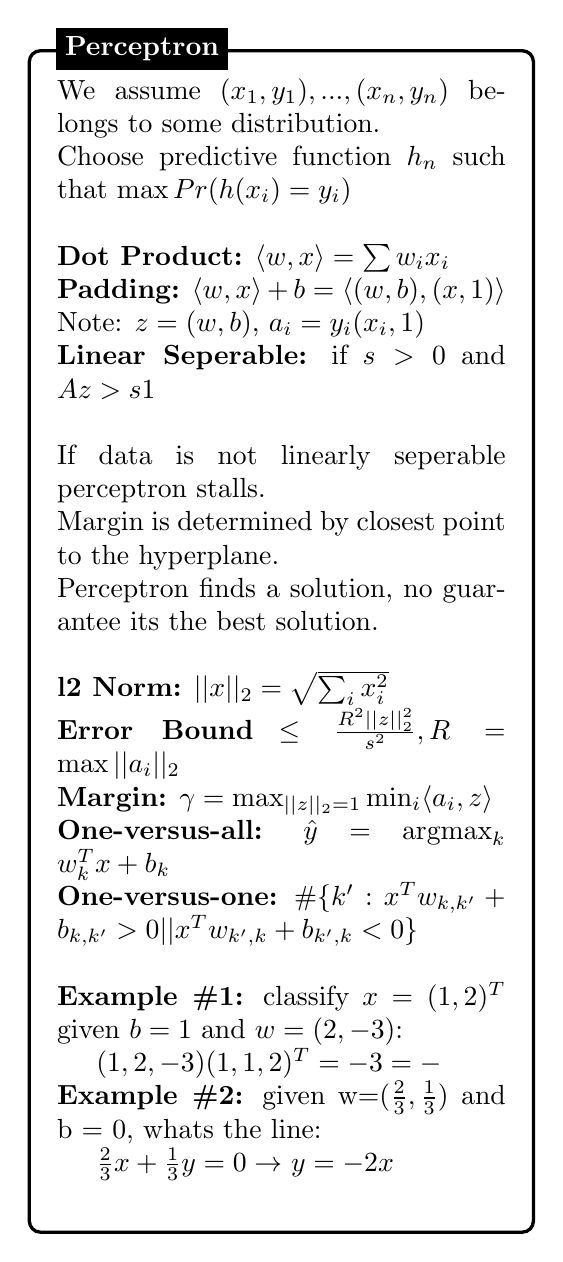
\begin{tikzpicture}
\node [mybox] (box){%
    \begin{minipage}{0.47\textwidth}
    We assume $(x_1,y_1),...,(x_n,y_n)$ belongs to some distribution.\\
    Choose predictive function  $h_n$ such that $\max Pr(h(x_i) = y_i)$ \\
    
    \textbf{Dot Product:} $ \langle w, x  \rangle = \sum w_ix_i $\\
    \textbf{Padding:} $\langle w, x  \rangle + b = \langle (w, b), (x, 1) \rangle$ \\
    Note: $z = (w,b)$, $a_i = y_i(x_i,1)$\\
    \textbf{Linear Seperable:} if $s>0$ and $Az > s1$ \\
    
If data is not linearly seperable perceptron stalls. \\
Margin is determined by closest point to the hyperplane. \\
Perceptron finds a solution, no guarantee its the best solution. \\

    \textbf{l2 Norm:} $||x||_2 = \sqrt{\sum_ix_i^2}$ \\
    \textbf{Error Bound} $\leq \frac{R^2||z||^2_2}{s^2}, R = \max||a_i||_2$  \\
    \textbf{Margin:} $\gamma = \max_{||z||_2 = 1} \min_i \langle a_i, z \rangle$ \\
    \textbf{One-versus-all:}  $\hat{y} = \text{argmax}_k$ $w_k^Tx + b_k $ \\
    \textbf{One-versus-one:} $\# \{k' : x^Tw_{k,k'} + b_{k,k'} > 0 || x^Tw_{k',k} + b_{k',k} < 0 \}$\\
    
    \textbf{Example \#1:} classify $x = (1,2)^T$ given $b=1$ and $w=(2,-3)$:\\
     \blank{0.5cm}$ (1, 2, -3) (1, 1, 2)^T = -3 = -$ \\
     \textbf{Example \#2:} given w=($\frac{2}{3}, \frac{1}{3}$) and b = 0, whats the line: \\
     \blank{0.5cm}$ \frac{2}{3}x + \frac{1}{3}y = 0 \rightarrow$ $y = -2x$ \\
    \end{minipage}
};
\node[fancytitle, right=10pt] at (box.north west) {Perceptron};
\end{tikzpicture}

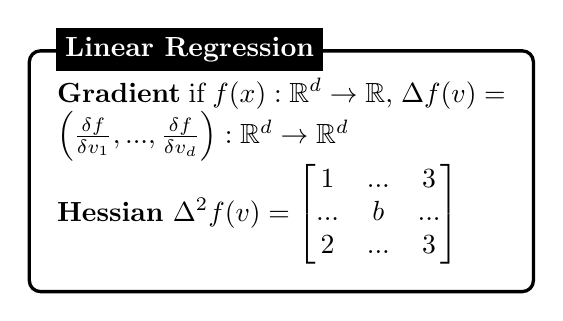
\begin{tikzpicture}
\node [mybox] (box){%
    \begin{minipage}{0.47\textwidth}
	\textbf{Gradient} if $f(x): \mathbb{R}^d \rightarrow \mathbb{R}$, $\Delta f(v) = \left( \frac{\delta f}{\delta v_1}, ..., \frac{\delta f}{\delta v_d}  \right): \mathbb{R}^d \rightarrow \mathbb{R}^d$ \\
	\textbf{Hessian} $\Delta^2 f(v) = \begin{bmatrix}
1 & ... & 3 \\
... & b & ... \\
2 & ... & 3
\end{bmatrix}$
    \end{minipage}
};
\node[fancytitle, right=10pt] at (box.north west) {Linear Regression};
\end{tikzpicture}
\end{multicols*}

\end{document}